% !TEX root = ../../Main.tex
\section{Trading Behaviour: How the Agents Actually Trade}
\label{Section:TradingBehaviour}

A return figure says whether an agent made money. It says nothing about how, and here that matters for a specific reason. The main claim of this work is that a continuous action lets one decision set both the direction and the size of a position. If the agents had learned to use only the two ends of that action, they would be discrete traders with extra machinery, and the claim would mean nothing. This section examines what they did in practice.

\subsection{Use of the Continuous Action}

The agent outputs an action $a \in [-1, 1]$ and holds $|a|$ of the reference size defined in \Cref{Equation:PositionSizing}. \Cref{Figure:ActionDistribution} shows how this value is distributed over the whole evaluation window for each pair.

% !TEX root = ../Main.tex
\begin{table}[htb!]
\centering
\footnotesize
\caption{Trading behaviour over the evaluation window. Mean $|a|$ is the average absolute action, that is, the average fraction of the reference position size held while in the market. Win rate is the share of closed positions with a positive net result after costs.}
\label{Tables:Behaviour}
\begin{tabular}{@{}lrrrrrr@{}}
\toprule
\textbf{Pair} & \textbf{Positions} & \textbf{Long} & \textbf{Median Hold} & \textbf{Longest Hold} & \textbf{Win Rate} & \textbf{Mean $|a|$} \\
\midrule
AUD/USD & 1,561 & 27.9\% & 9.7 d & 227 d & 52.7\% & 0.77 \\
EUR/USD & 1,778 & 55.5\% & 3.9 d & 43 d & 51.9\% & 0.40 \\
GBP/USD & 2,516 & 46.9\% & 12.6 d & 149 d & 51.3\% & 0.89 \\
NZD/USD & 1,011 & 24.0\% & 5.9 d & 119 d & 52.8\% & 0.24 \\
USD/CAD & 2,213 & 65.6\% & 5.7 d & 97 d & 55.0\% & 0.79 \\
USD/CHF & 220 & 34.2\% & 8.0 d & 345 d & 49.8\% & 0.09 \\
USD/JPY & 1,438 & 100.0\% & 2,120 d & 4,004 d & 50.7\% & 0.98 \\
\bottomrule
\end{tabular}
\end{table}

\begin{figure}[htb!]
\centering
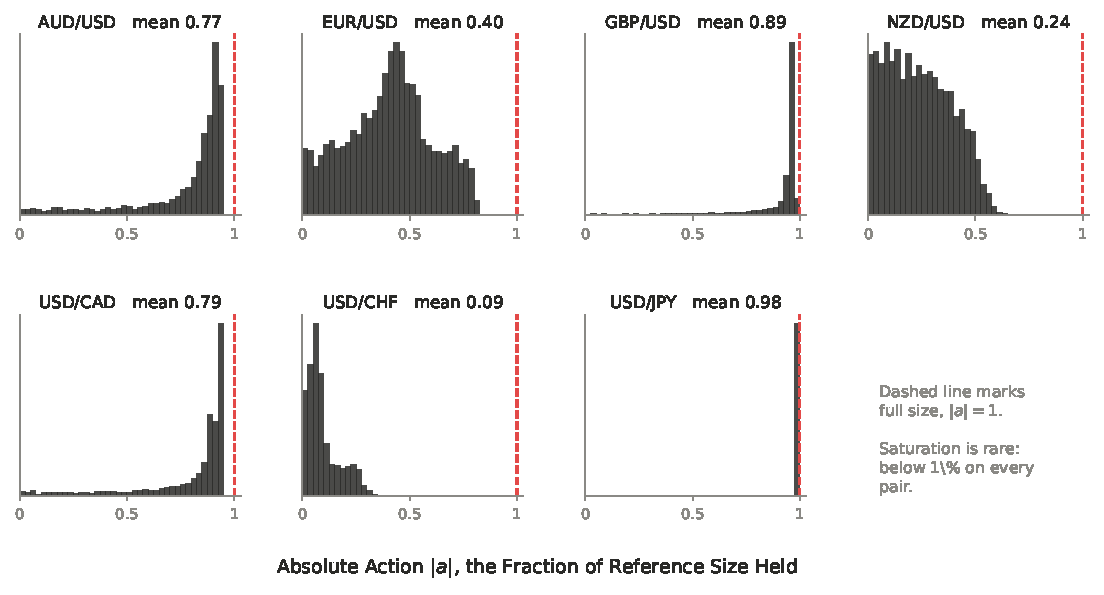
\includegraphics[width=\textwidth]{Images/ActionDistribution.pdf}
\caption{Distribution of the absolute action over the evaluation window. The dashed line marks full size. If the agents had turned the continuous action into a discrete one, these histograms would be concentrated against that line. Instead, most of the mass lies inside the range.}
\label{Figure:ActionDistribution}
\end{figure}

The action does not saturate at $+1$ or $-1$. On every pair, fewer than one percent of decisions are above $|a| = 0.98$, and on six of the seven pairs the figure is zero to one decimal place. The mean absolute action goes from $0.09$ on USD/CHF to $0.98$ on USD/JPY. The agents therefore settled on very different position sizes from the same design and the same reference risk.

This dispersion of sizes is informative in itself. USD/CHF holds roughly a tenth of the size available to it. This is why its maximum drawdown is $8.2\%$ while its Sharpe ratio is the highest of the seven. It found a small advantage and kept its size small to match, instead of pushing it harder. NZD/USD, at $0.24$, behaves in a similar way. USD/JPY is at the other end, with $0.98$. This number is the symptom of the failure described in \Cref{Section:NegativeResult}: an agent that always holds full size in one direction no longer makes a sizing decision at all.

The sizing also adapts in a second way, which the histogram does not show. The reference size is inversely proportional to the average true range, so the same action gives a smaller position when volatility rises. The action and the volatility scaling combine, and the position held is the product of the two.

\subsection{Direction, Size and Outcome Together}

\Cref{Figure:DecisionAnatomy} follows EUR/USD over three years. It shows the price, the action of the agent, the position it held as a result, and the equity that followed.

\begin{figure}[htb!]
\centering
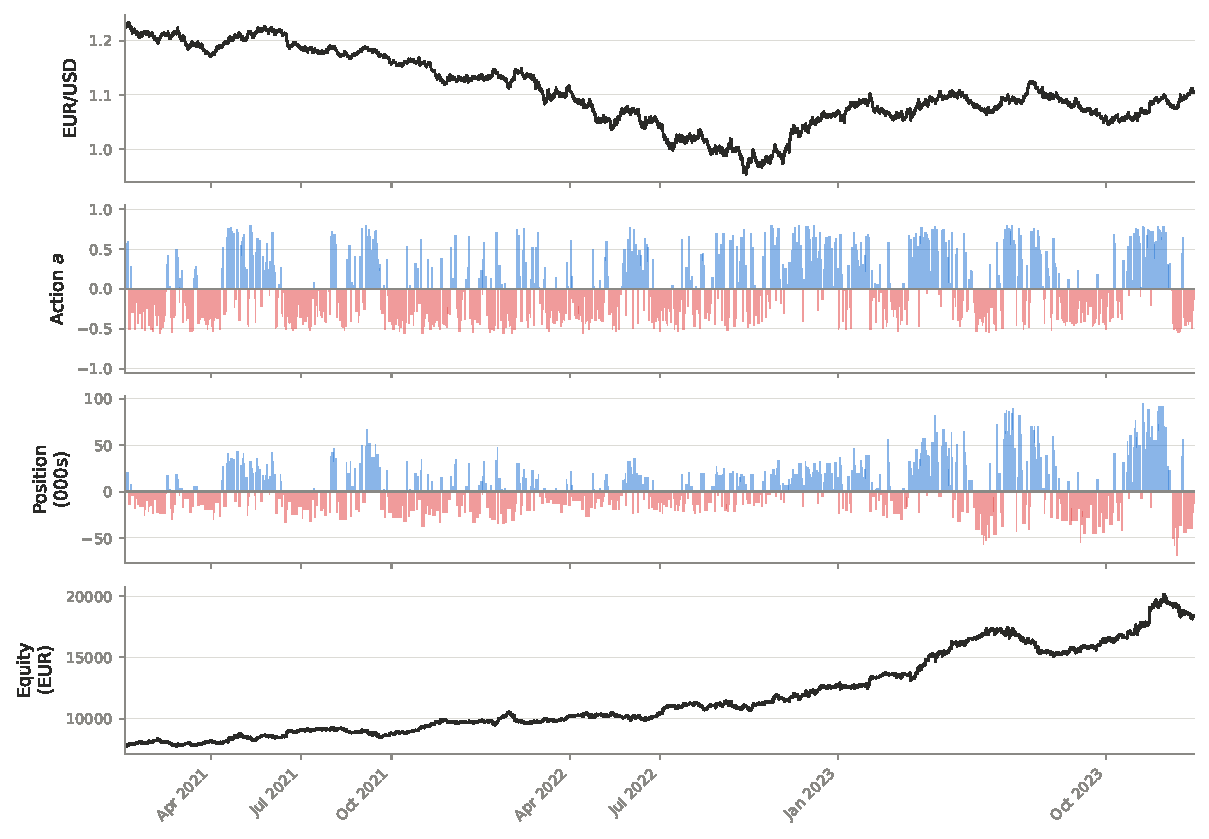
\includegraphics[width=\textwidth]{Images/DecisionAnatomy.pdf}
\caption{EUR/USD from 2021 to 2024. From top: the price; the action, positive for long and negative for short; the resulting net position in thousands of units; and account equity. The action changes sign well before the position does, because a change is only acted on when it is larger than the threshold of \Cref{Equation:Hysteresis}.}
\label{Figure:DecisionAnatomy}
\end{figure}

Three behaviours can be seen. First, the action moves continuously and does not switch between fixed levels. Its magnitude changes as much as its sign. Second, the position follows the action, but in larger steps, because the rebalance threshold blocks small adjustments. Long periods of constant position are periods where the agent kept changing its target by less than the threshold. Third, the sign does not change often. Over the three years the agent reverses direction a few dozen times. This fits the daily decision frequency, and does not fit an agent that reacts to every bar it observes.

\subsection{Trend Identification and Reversal}

The clearest example of an agent holding a position through a sustained move is GBP/USD in the second half of 2022, shown in \Cref{Figure:TrendRide}. Sterling fell from $1.22$ to below $1.04$ over roughly ten weeks, a fall of more than fifteen percent. The steepest part came after the United Kingdom fiscal announcement of late September.

\begin{figure}[htb!]
\centering
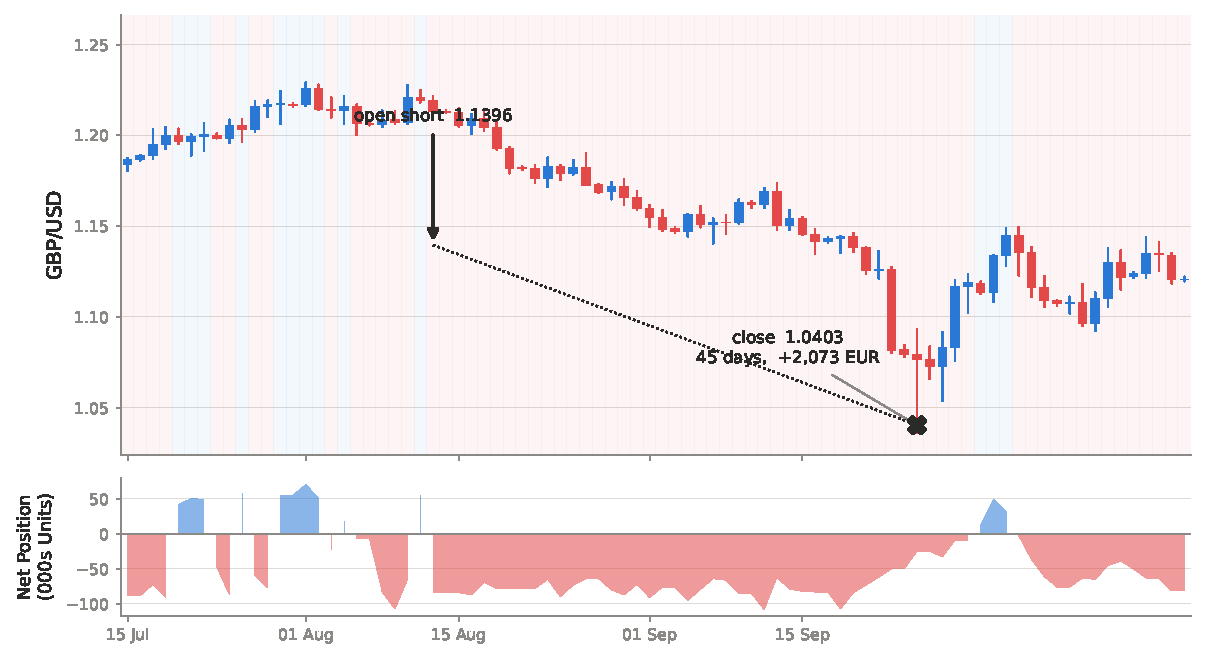
\includegraphics[width=\textwidth]{Images/TrendRide.pdf}
\caption{GBP/USD from mid-July to mid-October 2022. Background shading marks the direction of the net position, red for short and blue for long. The lower panel gives the size of that position. The marked trade is the most profitable single position of the eleven years on this pair.}
\label{Figure:TrendRide}
\end{figure}

The agent was short for almost the whole fall. It held short exposure of between fifty and one hundred thousand units, added to it as the move continued, and reduced it as the price neared the low. The marked position was opened at $1.1396$ on 12 August and closed at $1.0403$ on 26 September, forty-five days later. Its net profit was $2\,073$ euros after costs. It is the largest single position of the eleven years on this pair.

Two details are worth pointing out, because they show judgement and not luck. The agent was briefly long at the end of July, at the local high before the fall began. It was long again in the days right after the bottom. Both times the size was small. It did not hold the short position forever. Once the price recovered above $1.12$ in early October, the position was reduced and then reversed. This is how an agent behaves when it responds to the state it observes, and not when it is fixed on one direction.

\subsection{Holding Periods and Two-Sided Exposure}

\Cref{Tables:Behaviour} gives the trading statistics for each pair, and \Cref{Figure:HoldingBehaviour} shows two of them. Median holding periods go from four days on EUR/USD to nearly thirteen on GBP/USD, and the longest single positions last for months. These agents are swing traders, which hold positions for days, and not scalpers, which trade in and out quickly. This is what the daily decision frequency of \Cref{Section:ExperimentalProcedure} was meant to produce.

\begin{figure}[htb!]
\centering
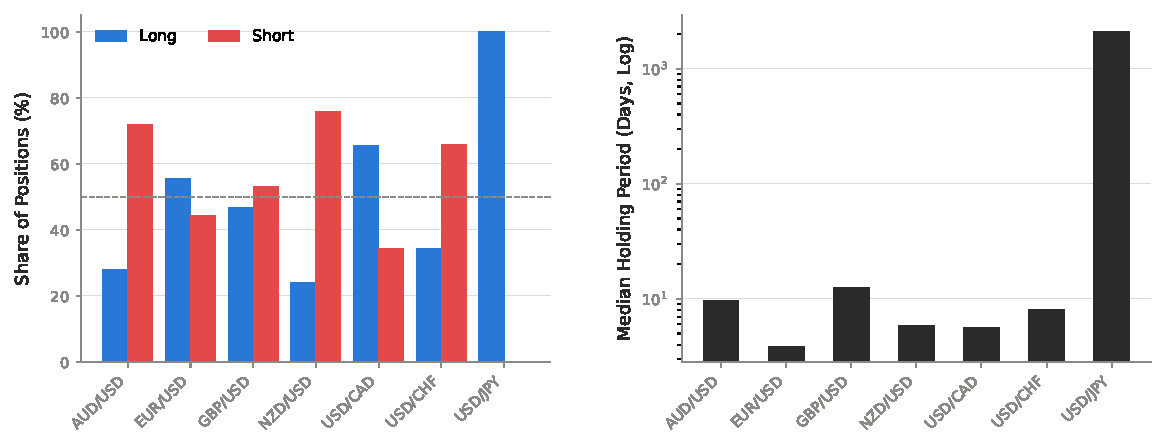
\includegraphics[width=\textwidth]{Images/HoldingBehaviour.pdf}
\caption{Left: the share of positions taken long and short. Right: the median holding period in days, on a logarithmic scale. USD/JPY is long in every position it takes and holds for years, which puts it far outside the range of the other six.}
\label{Figure:HoldingBehaviour}
\end{figure}

The long and short shares differ a lot between pairs, from $24\%$ long on NZD/USD to $66\%$ on USD/CAD. EUR/USD and GBP/USD are close to balanced. None of the six working agents trades only one side. This comes from the design and is not an accident. The eligibility test of \Cref{Section:ExperimentalProcedure} rejected any episode whose weaker side fell below a threshold, so a one-sided policy could not be selected, however profitable it looked. USD/JPY is the exception, at $100\%$ long. It is the exception because none of the $448$ seeds that were tried on that pair could pass that test.

\subsection{Where the Profit Comes From}

One statistic in \Cref{Tables:Behaviour} deserves a closer look. The win rate is the fraction of positions closed at a profit. It lies between $49.8\%$ and $55.0\%$ across the seven pairs. Six of the seven are within three points of a coin toss. USD/CHF, the best model of the seven on every risk measure, has the lowest win rate of all, at $49.8\%$.

So the agents do not make money by being right more often than they are wrong. Their profit comes from what they do with a position once it is open. They hold a larger size when the position moves in their favour than when it does not, and they keep positions that work open longer than positions that do not. A continuous action makes this possible. An agent that can only choose a direction cannot do it. This also explains how USD/CHF can be the strongest model of the seven while being wrong slightly more often than a coin toss. It trades at small size and is patient, and the few positions it holds at a larger size are the ones that worked.

\subsection{What the Trading Costs}

The engine charges the spread quoted at each fill and a real commission schedule. The difference between what the policies earned and what the account kept can therefore be measured, and does not have to be estimated.

The commission is recorded directly on every trade. The spread is not, because it is paid inside each fill and is not deducted afterwards. A buy is filled at the ask and a sell at the bid, so the cost is already included in the entry and exit prices. It can still be recovered exactly, because the two charges scale in the same way. Commission is charged at $3.5$ points per side, which is seven points for a round turn, that is, one opening and one closing trade. The spread is crossed once per round turn. Both are proportional to the traded volume, and both are converted into the account currency at the same rate. So for any position

\begin{equation}
C_{spread} = \left| C_{commission} \right| \cdot \frac{s}{7}
\label{Equation:SpreadRecovery}
\end{equation}

where $s$ is the spread in points at the moment of the trade. Applying \Cref{Equation:SpreadRecovery} to every position gives \Cref{Tables:Costs}, with $s$ taken from the recorded quotes for the month in which the position was opened.

% !TEX root = ../Main.tex
\begin{table}[htb!]
\centering
\footnotesize
\caption{What the seven agents earned before costs and what they kept, in euros. Cost share is the spread and the commission together, as a fraction of profit before costs. The mean spread column is the commission-weighted average spread paid, in points. It differs from the pair's average spread because it gives weight to the moments when the agent traded.}
\label{Tables:Costs}
\begin{tabular}{@{}lrrrrrr@{}}
\toprule
\textbf{Pair} & \textbf{Before Costs} & \textbf{Spread} & \textbf{Commission} & \textbf{Net} & \textbf{Cost Share} & \textbf{Mean Spread} \\
\midrule
AUD/USD & 11,851 & $-1,162$ & $-2,200$ & 8,488 & 28.4\% & 3.70 pts \\
EUR/USD & 9,372 & $-638$ & $-1,669$ & 7,064 & 24.6\% & 2.68 pts \\
GBP/USD & 19,086 & $-2,456$ & $-3,168$ & 13,462 & 29.5\% & 5.43 pts \\
NZD/USD & 8,552 & $-1,238$ & $-1,424$ & 5,890 & \textbf{31.1\%} & 6.09 pts \\
USD/CAD & 28,272 & $-2,695$ & $-3,432$ & 22,145 & 21.7\% & 5.50 pts \\
USD/CHF & 5,735 & $-148$ & $-130$ & 5,457 & \textbf{4.8\%} & 7.93 pts \\
USD/JPY & 2,172 & $-411$ & $-155$ & 1,606 & 26.1\% & 18.53 pts \\
\midrule
\textbf{Total} & \textbf{85,039} & $\mathbf{-8,748}$ & $\mathbf{-12,179}$ & \textbf{64,112} & \textbf{24.6\%} & --- \\
\bottomrule
\end{tabular}
\end{table}

The seven agents earned $85\,039$ euros before costs and kept $64\,112$. Of the difference, $8\,748$ euros went to the spread and $12\,179$ to commission, so \textbf{costs took $24.6\%$ of trading profit}. Commission is the larger of the two charges here because the account is a raw-spread account. On such an account the spread is narrow by design, and the broker makes its money through the commission instead. On an account with wider spreads and no commission, the same trades would have paid a similar total, split in a different way.

\Cref{Tables:Costs} has no swap column because the swap is zero on every pair. A swap-free account charges no overnight financing, so zero is the exact figure and not an approximation. This matters at these holding periods. Agents that hold positions for a median of four to thirteen days would otherwise pay financing on several hundred nights each.

The differences between pairs are large, and they follow turnover almost exactly. USD/CHF takes $220$ positions and gives up $4.8\%$ of its profit before costs, so it keeps more than nineteen euros in every twenty. NZD/USD gives up $31.1\%$ and GBP/USD $29.5\%$. A policy of the same quality therefore gives very different net results at different trading frequencies. This is why the selection criteria of \Cref{Section:ExperimentalProcedure} reward long holding periods directly, instead of relying on the return figure to include this effect. It is also why the rebalance threshold of \Cref{Equation:Hysteresis} contributes as much as \Cref{Tables:Deployment} shows.

One consequence matters for how the rest of this chapter should be read. Every return quoted in this work is net of both charges. A study that tested the same policies on bar closes with no spread and no commission would have reported the before-costs column of \Cref{Tables:Costs}. That column is a third larger, and it describes a strategy that no account could have traded.

Recovering the spread through \Cref{Equation:SpreadRecovery} works, but it is indirect and it needs a commission that is not zero. The engine computes the spread charge internally when it opens a position. It does not yet write this charge to the exported trade record as a separate field. Recording it there, next to commission and swap, is a simple improvement and is noted in \Cref{Section:FutureWork}.